\documentclass{article}
\usepackage[utf8]{inputenc}

\title{MI-PAA: Problém batohu, úloha 2}
\author{Josef Doležal}

\usepackage{natbib}
\usepackage[czech]{babel}
\usepackage{a4wide}
\usepackage{graphicx}

\graphicspath{{reports/report-02/}}

\begin{document}

\maketitle

\section{Úvod}
Problémem batohu se nazývá úloha, ve které je za úkol pro množinu $n$ předmětů a batoh o maximální nosnosti $m$ určit, jak předměty do batohu vložit tak, aby v součtu měly co největší hodnotu a zároveň nebyla překročena maximální nosnost batohu.

Vstupem je tedy seznam $n$ předmětů (dvojic váha-cena) a maximální nosnost batohu $m$.
Výstupem je v součtu nejvyšší možná cena předmětů, jejichž váha dohromady nepřekročí nosnost.

\section{Zadání úlohy}

\begin{itemize}
    \item Naprogramujte řešení problému batohu:
    
    \begin{enumerate}
        \item metodou větví a hranic (B\&B) tak, aby omezujícím faktorem byla hodnota optimalizačního kritéria. Tj. použijte ořezávání shora (překročení kapacity batohu) i zdola (stávající řešení nemůže být lepší než nejlepší dosud nalezené),
        
        \item metodou dynamického programování (dekompozice podle kapacity nebo podle cen),
        
        \item FPTAS algoritmem, tj. s použitím modifikovaného dynamického programování s dekompozicí podle ceny (při použití dekompozice podle kapacity není algoritmus FPTAS).
    \end{enumerate}
\end{itemize}

\section{Rámcový popis řešení}

Zadání úlohy specifikuje vyřešit problém pomocí metody větví a hranic, pomocí dynamického programování a aproximačního přístupu FPTAS.
K implementaci jednotlivých algoritmů je využit programovací jazyk Swift.

Jednotlivé algoritmy jsou implementovány pomocí tříd implementujících protokol (ekvivalent \texttt{Interface} používaného v jazyce Java) nazvaný \texttt{FittingStrategyType}. Tento protokol vyžaduje po objektech, kterého implementují, existenci statické metody\\
\texttt{fit(items: maxWeight:) -> BackpackFittingResult?}.

Metody řešení jsou implementovány pomocí rekurze.
Při výpočtu pomocí dynamického programování je využita dekompozice podle ceny.

Pro každou instanci program vyřeší problém všemi požadovanými postupy samostatně.
Pro všechna řešení program změří procesorový čas, který byl potřebný k získání výsledku.
Výsledky jsou poskytovány jako datový vstup pro program Gnuplot a \LaTeX{}.

\section{Popis algoritmu}

V této části rozebírám konkrétní implementaci jednotlivých řešení.
Součástí popisů jsou grafy, znázorňující časovou závislost na počtu předmětů.

\subsection*{Metoda větví a hranic}

Metoda větví a hranic je optimalizační algoritmus, který urychluje výpočet algoritmu hrubé síly.

Optimalizace spočívá ve vynechávání takových kombinací prvků batohu, které nemohou dohromady vytvořit optimální řešení. V prvním kroku algoritmus seřadí prvky podle poměru cena/hmotnost.

V každém dalším kroce následně algoritmus vezme prvek ze seznamu a rozvětví se na možnost kdy prvek v batohu je a kdy není. Vrámci tohoto kroku se navíc kontroluje, jestli je nutné tyto větve procházet. K tomu se využívají hranice. Horní hranicí je cena. Algoritmus pro celý výpočet udržuje v paměti nejlepší nalezené řešení - pokud je v průchodu větev, která má v nejlepším případě nižší hodnotu než je aktuální maximum, větev se neprochází.
Spodní hranicí je váha. Pokud se během větvení stane, že přidáním následujícího prvku bychom přesáhli kapacitu batohu, větev se neprochází.

Jakmile se algoritmus dostane větvením až k poslednímu prvku seznamu a zároveň je v součtu hodnota obsažených prvků maximální, aktualizuje se globální maximum.

Algoritmus je tedy rekurzivní, v každém kroce se udržuje aktuální cena vložených prvků, zbývající kapacita batohu a maximální možné ohodnocení větve. První prvek seznamu má ohodnocení obou podvětví jako součet cen všech prvků batohu. V rekurzivním volání je maximální cena podvětví snížena o cenu prvku. Pokud byl navíc prvek vložen, zvýší se aktuální cena batohu a zároveň se sníží jeho maximální nosnost.

Stejně jako u algoritmu hrubé síly je i zde v nejhorším případě nutné projít všechny kombinace.

\begin{figure}[ht]
    \centering
    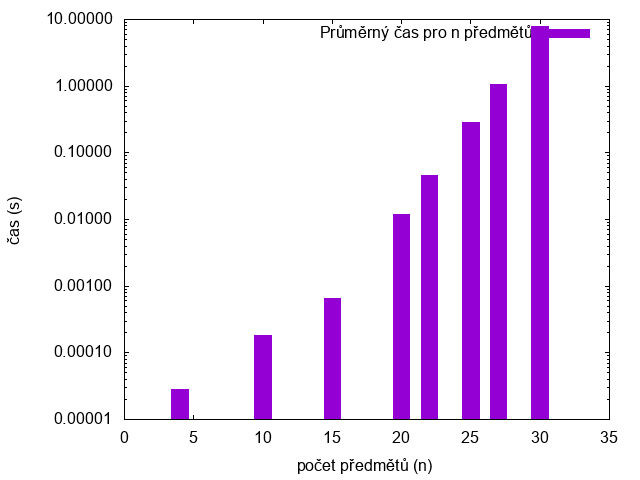
\includegraphics[width=0.8\textwidth]{bb-duration.png}
    \caption{[B\&B] Průměrný čas pro 50 instancí a $n$ předmětů}
    \label{fig:g1}
\end{figure}

Z obrázky \ref{fig:g1} je vidět, že čas pro řešení roste exponencionálně.
Vzhledem k velkému nárustu času je osa Y logaritmicky škálovaná.
Časy jsou ovšem oproti metodě hrubé síly, kde už pro více než 25 prvků byl čas výpočtu neúnosný (cca 1h pro vypočtení instance) mnohem přijatelnějíší.

\subsection*{Dynamické programování}

Metoda dynamického programování je další optimalizační metodou hledání řešení.
Hledání řešení spočívá ve vyplňování tabulky.
Tento algoritmus se totiž snaží časovou složitost přeměnit v paměťovou.

Velikost a formát tabulky se odvíjí od zvolené strategie.
Možné je využít dekompozici podle ceny nebo podle váhy.
Ve své implementaci jsem využil dekompozici podle ceny, kterou jsem následně také využil k implementaci aproximačního řešení pomocí FPTAS.

Implementace spočívá ve vytvoření tabulky, která v záhlaví řádků obsahuje prvky batohu a v záhlaví sloupců cenu v intervalu $(0, k]$, kde $k$ je součet cen všech položek.

\begin{figure}[ht]
    \centering
    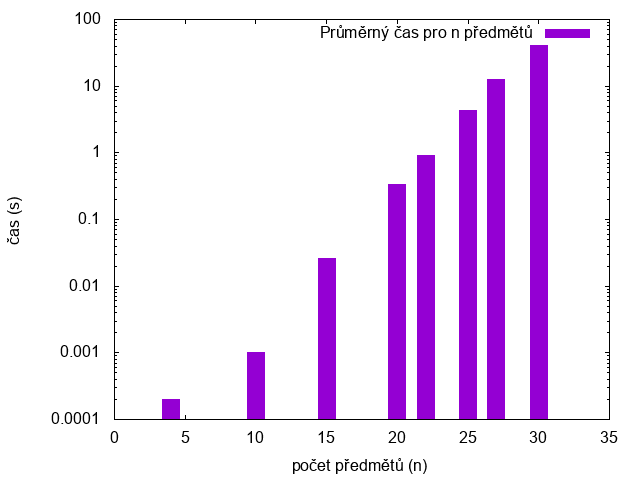
\includegraphics[width=0.8\textwidth]{dynamic-programming-duration.png}
    \caption{[Dynamické programování] Průměrný čas pro 50 instancí a $n$ předmětů}
    \label{fig:g2}
\end{figure}

Algoritmus postupně vyplňuje tabulku a do každé buňky vkládá nejmenší možnou hmotnost, které se mu podařilo dosáhnout při průchodu.
V prvním kroku začíná algoritmus v bodě $(x, y) := (0, 0)$.
Algoritmus se podobně jako v metodě větví a hranic rozděluje na dvě části, tedy jestli je prvek ve výsledku obsažen či nikoli.
Pro případ kdy není se přesouvá algoritmus dále na pole $(x, y+1)$.
V případě že prvek bude ve výsledku obsažený, přesouvá se algoritmus na pole $(cena, y+1)$, současně se zvyšuje aktuální cena a hmotnost batohu. Do pole tabulky se pak zapisuje altuální hmotnost batohu, pokud se v poli současně nevyskytuje nižší hodnota.

Jak je vidět z grafu \ref{fig:g1} a \ref{fig:g2}, algoritmus má obdobnou složitost jako metoda větví a hranic, pro většinu instancí je však doba výpočtu až čtyřikrát vyšší.

Algoritmus pracuje v pseudopolynomiálním čase se složitostí $O(K \cdot n)$, jeho složitost jde tedy omezit polynomem vzhledem k délce vstupu (počet předmětů) ale ne k velikosti vstupu ($K$ - cena - může být až exponenciální).

\subsection*{FPTAS}

Aproximační algoritmus FPTAS (Fully Polynomial-Time Approximation Scheme) je upravenou verzí algoritmu pro dynamické programování. Tato metoda se pomocí zavedení odchylky snaží redukovat časovou ale i paměťovou složitost algoritmu.

Snížení paměťové složitosti je docíleno snížením cen položek batohu.
Každá položka je před výpočtem pronásobena koeficientem $k = e \cdot \frac{v_i}{n}$, kde $e$ udává požadovanou přesnost, $v_i$ je cena cena $i$-té položky na vstupu a $n$ je počet prvků na vstupu.

Přesnost výpočtu se algoritmu zadává pomocí maximální přípustné odchylky.
Po úpravě cen položek batohu přichází na řadu opět dynamické programování, které na vstup dostává seznam položek s upravenou cenou.

\begin{figure}[ht]
    \centering
    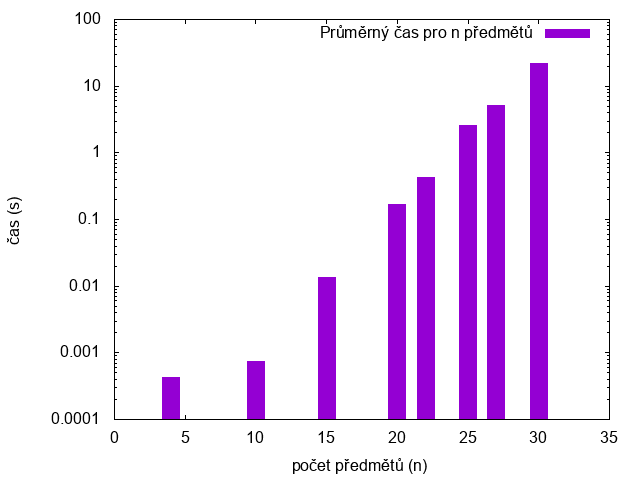
\includegraphics[width=0.8\textwidth]{fptas-duration.png}
    \caption{[FPTAS]Průměrný čas pro 50 instancí a $n$ předmětů (e = 0.1)}
    \label{fig:g3}
\end{figure}

Graf \ref{fig:g3} znázorňuje podobný trend růstu časové složitosti jako metoda větví a hranic.
I v tomto případě ale s rostoucím $n$ metoda větví a hranic působí nepatrněji rychleji.
Srovnání všech zmíněných metod je znázorněn v grafu \ref{fig:g4}.

\begin{figure}[ht]
    \centering
    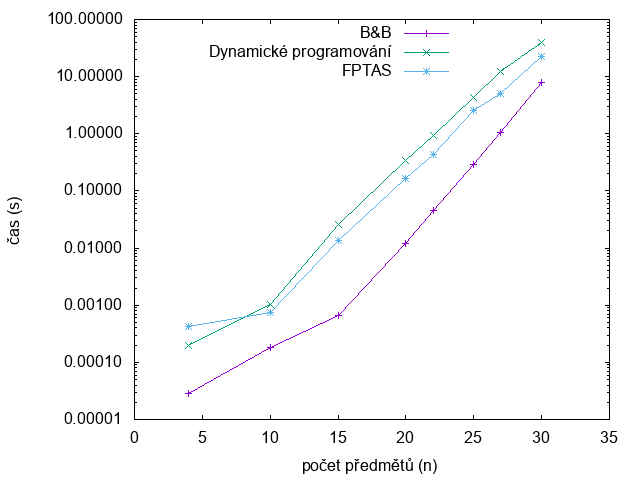
\includegraphics[width=0.8\textwidth]{multiplot.png}
    \caption{[FPTAS] Porovnání průměrných časů všech implementovaných metod}
    \label{fig:g4}
\end{figure}

\subsubsection*{Chyba výpočtu}

Aproximační řešení problému vnáší do řešení možnost chyby.
Při měření metody FPTAS jsem sledoval průměrnou a maximální odchylku vypočteného řešení od optimálního.

Měření jsem opakoval pro různá $e$ znázorňující přesnost.
Pro $e := 0.1$ (přesnost $10 \%$), $e := 0.3$ a $e := 0.9$.
S rostoucí vyžadovanou přesností jsem vysledoval pokles optimalizace a algoritmus se přibližoval svou rychlostí k metodě dynamického programování.

\begin{figure}[ht]
    \centering
    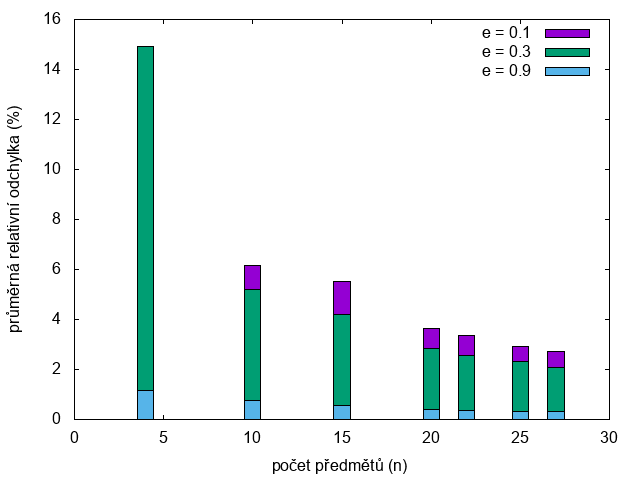
\includegraphics[width=0.8\textwidth]{average-error.png}
    \caption{Průměrná relativní odchylka pro 50 instancí a $n$ předmětů s přesností $e$}
    \label{fig:g5}
\end{figure}

Jak je patrné z grafu \ref{fig:g5} a \ref{fig:g6}, průměrná i relativní chyba se zmenšují pro rostoucí $n$.
Přesnost algoritmu je také více patrná na menších instancích, pro 27 prvků maximální chyba žádné z metod nepřesáhla $5 \%$.

\begin{figure}[ht]
    \centering
    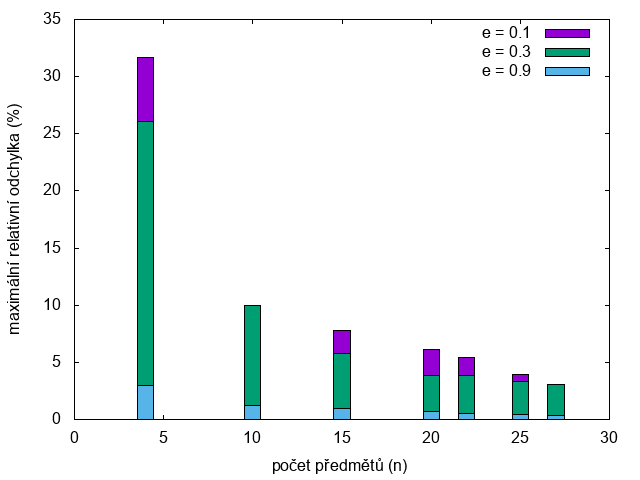
\includegraphics[width=0.8\textwidth]{max-error.png}
    \caption{Maximální relativní odchylka pro 50 instancí a $n$ předmětů s přesností $e$}
    \label{fig:g6}
\end{figure}

\section{Závěr}

Z naměřených dat lze usoudit, že nejrychlejším algoritmem je metoda větví a hranic, která pro všechny instance trvala nejkratší dobu.
Tato metoda je ale z pozorování nejvíce datově citlivá. Jako jediná z měřených totiž trpěla extrémními výkyvy od naměřeného průměru.
To je dáno tím, že pro určité vstupy se optimalizace pomocí hranic neprojeví tak výrazně a je nutné projít větší část statového prostoru.

Obě exaktní metody (větve a hranice, dynamické programování) jsou oproti metodě hrubé síly podstatným zlepšením.

Aproximační metoda proti všem očekávání nepřinesla podstatné zlepšení oproti exaktním metodám.
Přestože s rostoucím počtem položek v batohu chyba tohoto algoritmu klesá, vyplatí se stále využít exaktní metodu větví a hranic, která je rychlejší a poskytuje přesný výsledek.

Zajímavým pozorováním je velikost maximální chyby.
Ta se pro $n >= 20$ snížila pod $5 \%$ pro všechny měřené přesnosti.
Pokud je tedy $n$ vysoké a zároveň se spokojíme s přesností v řádech menších jednotek procent, nemusíme po algoritmu vyžadovat vysokou přesnost explicitně.

Efektivita algoritmu dynamického programování může být ovlivněna konkrétní implementací.
Při implementaci větví a hranic jsem se více zaměřil na paměťovou náročnost rekurzivních volání, což může značným způsobem výsledek ovlivnit.

\end{document}
